\begin{figure}[htbp]
\centering
\begin{minipage}{0.46\textwidth}\centering
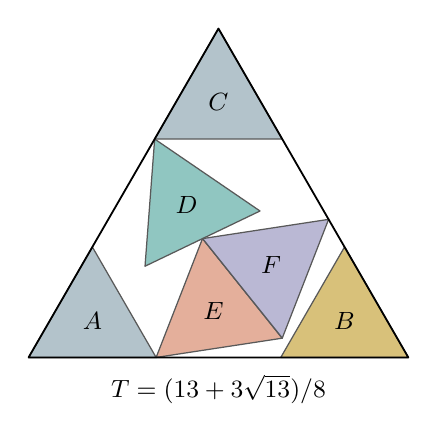
\begin{tikzpicture}[x=1.62cm,y=1.62cm,line join=round]
\definecolor{pieceA}{HTML}{6d8c9b}
\filldraw[fill=pieceA,fill opacity=0.52,draw=black!65,line width=.45pt] (0.000000000,0.000000000) -- (1.000000000,0.000000000) -- (0.500000000,0.866025404) -- cycle;
\node[font=\small] at (0.500000000,0.288675135) {$ A $};
\definecolor{pieceB}{HTML}{b58900}
\filldraw[fill=pieceB,fill opacity=0.52,draw=black!65,line width=.45pt] (1.977081728,0.000000000) -- (2.977081728,0.000000000) -- (2.477081728,0.866025404) -- cycle;
\node[font=\small] at (2.477081728,0.288675135) {$ B $};
\definecolor{pieceC}{HTML}{6d8c9b}
\filldraw[fill=pieceC,fill opacity=0.52,draw=black!65,line width=.45pt] (0.988540864,1.712203002) -- (1.988540864,1.712203002) -- (1.488540864,2.578228406) -- cycle;
\node[font=\small] at (1.488540864,2.000878137) {$ C $};
\definecolor{pieceD}{HTML}{2a9188}
\filldraw[fill=pieceD,fill opacity=0.52,draw=black!65,line width=.45pt] (0.912846955,0.715071901) -- (1.814234774,1.148084603) -- (0.988540864,1.712203002) -- cycle;
\node[font=\small] at (1.238540864,1.191786502) {$ D $};
\definecolor{pieceE}{HTML}{cb6640}
\filldraw[fill=pieceE,fill opacity=0.52,draw=black!65,line width=.45pt] (1.000000000,0.000000000) -- (1.988540864,0.150953502) -- (1.363540864,0.931578252) -- cycle;
\node[font=\small] at (1.450693909,0.360843918) {$ E $};
\definecolor{pieceF}{HTML}{7b77ad}
\filldraw[fill=pieceF,fill opacity=0.52,draw=black!65,line width=.45pt] (1.363540864,0.931578252) -- (1.988540864,0.150953502) -- (2.352081728,1.082531755) -- cycle;
\node[font=\small] at (1.901387819,0.721687836) {$ F $};
\draw[line width=.65pt] (0.000000000,0.000000000) -- (2.977081728,0.000000000) -- (1.488540864,2.578228406) -- cycle;
\node[below,font=\small] at (1.488540864,-.06) {$T=(13+3\sqrt{13})/8$};
\end{tikzpicture}\par\smallskip
(a) Attaining construction.
\end{minipage}\hfill
\begin{minipage}{0.46\textwidth}\centering
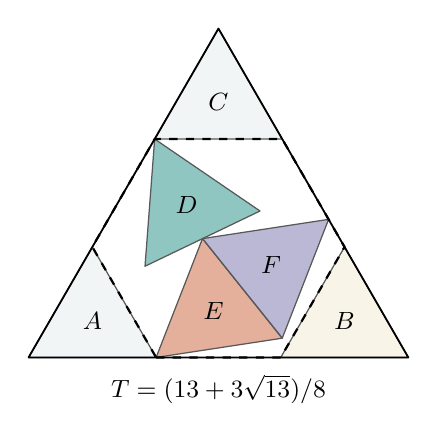
\begin{tikzpicture}[x=1.62cm,y=1.62cm,line join=round]
\definecolor{pieceA}{HTML}{6d8c9b}
\filldraw[fill=pieceA,fill opacity=0.09,draw=black!65,line width=.45pt] (0.000000000,0.000000000) -- (1.000000000,0.000000000) -- (0.500000000,0.866025404) -- cycle;
\node[font=\small] at (0.500000000,0.288675135) {$ A $};
\definecolor{pieceB}{HTML}{b58900}
\filldraw[fill=pieceB,fill opacity=0.09,draw=black!65,line width=.45pt] (1.977081728,0.000000000) -- (2.977081728,0.000000000) -- (2.477081728,0.866025404) -- cycle;
\node[font=\small] at (2.477081728,0.288675135) {$ B $};
\definecolor{pieceC}{HTML}{6d8c9b}
\filldraw[fill=pieceC,fill opacity=0.09,draw=black!65,line width=.45pt] (0.988540864,1.712203002) -- (1.988540864,1.712203002) -- (1.488540864,2.578228406) -- cycle;
\node[font=\small] at (1.488540864,2.000878137) {$ C $};
\definecolor{pieceD}{HTML}{2a9188}
\filldraw[fill=pieceD,fill opacity=0.52,draw=black!65,line width=.45pt] (0.912846955,0.715071901) -- (1.814234774,1.148084603) -- (0.988540864,1.712203002) -- cycle;
\node[font=\small] at (1.238540864,1.191786502) {$ D $};
\definecolor{pieceE}{HTML}{cb6640}
\filldraw[fill=pieceE,fill opacity=0.52,draw=black!65,line width=.45pt] (1.000000000,0.000000000) -- (1.988540864,0.150953502) -- (1.363540864,0.931578252) -- cycle;
\node[font=\small] at (1.450693909,0.360843918) {$ E $};
\definecolor{pieceF}{HTML}{7b77ad}
\filldraw[fill=pieceF,fill opacity=0.52,draw=black!65,line width=.45pt] (1.363540864,0.931578252) -- (1.988540864,0.150953502) -- (2.352081728,1.082531755) -- cycle;
\node[font=\small] at (1.901387819,0.721687836) {$ F $};
\draw[dashed,line width=.8pt] (1.000000000,0.000000000) -- (1.977081728,0.000000000) -- (2.477081728,0.866025404) -- (1.988540864,1.712203002) -- (0.988540864,1.712203002) -- (0.500000000,0.866025404) -- cycle;
\draw[line width=.65pt] (0.000000000,0.000000000) -- (2.977081728,0.000000000) -- (1.488540864,2.578228406) -- cycle;
\node[below,font=\small] at (1.488540864,-.06) {$T=(13+3\sqrt{13})/8$};
\end{tikzpicture}\par\smallskip
(b) The remaining hexagon $H(T)$.
\end{minipage}
\caption{The exact reference packing, drawn with rounded coordinates. The dashed cuts in (b) remove the three aligned unit corner interiors. The corner-replacement theorem applies to arbitrary packings; the depicted survivor triple is the reference example, not an assumed contact pattern.}\label{fig:construction}
\end{figure}
